\documentclass{ximera}
\graphicspath{  %% When looking for images,
{./}            %% look here first,
{./pictures/}   %% then look for a pictures folder,
{../pictures/}  %% which may be a directory up.
{../../pictures/}  %% which may be a directory up.
{../../../pictures/}  %% which may be a directory up.
{../../../../pictures/}  %% which may be a directory up.
}

\usepackage{listings}
%\usepackage{circuitikz}
\usepackage{xcolor}
\usepackage{amsmath,amsthm}
\usepackage{subcaption}
\usepackage{graphicx}
\usepackage{tikz}
%\usepackage{tikz-3dplot}
\usepackage{amsfonts}
%\usepackage{mdframed} % For framing content
%\usepackage{tikz-cd}

  \renewcommand{\vector}[1]{\left\langle #1\right\rangle}
  \newcommand{\arrowvec}[1]{{\overset{\rightharpoonup}{#1}}}
  \newcommand{\ro}{\texttt{R}}%% row operation
  \newcommand{\dotp}{\bullet}%% dot product
  \renewcommand{\l}{\ell}
  \let\defaultAnswerFormat\answerFormatBoxed
  \usetikzlibrary{calc,bending}
  \tikzset{>=stealth}
  




%make a maroon color
\definecolor{maroon}{RGB}{128,0,0}
%make a dark blue color
\definecolor{darkblue}{RGB}{0,0,139}
%define the color fourier0 to be the maroon color
\definecolor{fourier0}{RGB}{128,0,0}
%define the color fourier1 to be the dark blue color
\definecolor{fourier1}{RGB}{0,0,139}
%define the color fourier 1t to be the light blue color
\definecolor{fourier1t}{RGB}{173,216,230}
%define the color fourier2 to be the dark green color
\definecolor{fourier2}{RGB}{0,100,0}
%define teh color fourier2t to be the light green color
\definecolor{fourier2t}{RGB}{144,238,144}
%define the color fourier3 to be the dark purple color
\definecolor{fourier3}{RGB}{128,0,128}
%define the color fourier3t to be the light purple color
\definecolor{fourier3t}{RGB}{221,160,221}
%define the color fourier0t to be the red color
\definecolor{fourier0t}{RGB}{255,0,0}
%define the color fourier4 to be the orange color
\definecolor{fourier4}{RGB}{255,165,0}
%define the color fourier4t to be the darker orange color
\definecolor{fourier4t}{RGB}{255,215,0}
%define the color fourier5 to be the yellow color
\definecolor{fourier5}{RGB}{255,255,0}
%define the color fourier5t to be the darker yellow color
\definecolor{fourier5t}{RGB}{255,255,100}
%define the color fourier6 to be the green color
\definecolor{fourier6}{RGB}{0,128,0}
%define the color fourier6t to be the darker green color
\definecolor{fourier6t}{RGB}{0,255,0}

%New commands for this doc for errors in copying
\newcommand{\eigenvar}{\lambda}
%\newcommand{\vect}[1]{\mathbf{#1}}
\renewcommand{\th}{^{\text{th}}}
\newcommand{\st}{^{\text{st}}}
\newcommand{\nd}{^{\text{nd}}}
\newcommand{\rd}{^{\text{rd}}}
\newcommand{\paren}[1]{\left(#1\right)}
\newcommand{\abs}[1]{\left|#1\right|}
\newcommand{\R}{\mathbb{R}}
\newcommand{\C}{\mathbb{C}}
\newcommand{\Hilb}{\mathbb{H}}
\newcommand{\qq}[1]{\text{#1}}
\newcommand{\Z}{\mathbb{Z}}
\newcommand{\N}{\mathbb{N}}
\newcommand{\q}[1]{\text{``#1''}}
%\newcommand{\mat}[1]{\begin{bmatrix}#1\end{bmatrix}}
\newcommand{\rref}{\text{reduced row echelon form}}
\newcommand{\ef}{\text{echelon form}}
\newcommand{\ohm}{\Omega}
\newcommand{\volt}{\text{V}}
\newcommand{\amp}{\text{A}}
\newcommand{\Seq}{\textbf{Seq}}
\newcommand{\Poly}{\textbf{P}}
\renewcommand{\quad}{\text{    }}
\newcommand{\roweq}{\simeq}
\newcommand{\rowop}{\simeq}
\newcommand{\rowswap}{\leftrightarrow}
\newcommand{\Mat}{\textbf{M}}
\newcommand{\Func}{\textbf{Func}}
\newcommand{\Hw}{\textbf{Hamming weight}}
\newcommand{\Hd}{\textbf{Hamming distance}}
\newcommand{\rank}{\text{rank}}
\newcommand{\longvect}[1]{\overrightarrow{#1}}
% Define the circled command
\newcommand{\circled}[1]{%
  \tikz[baseline=(char.base)]{
    \node[shape=circle,draw,inner sep=2pt,red,fill=red!20,text=black] (char) {#1};}%
}

% Define custom command \strikeh that just puts red text on the 2nd argument
\newcommand{\strikeh}[2]{\textcolor{red}{#2}}

% Define custom command \strikev that just puts red text on the 2nd argument
\newcommand{\strikev}[2]{\textcolor{red}{#2}}

%more new commands for this doc for errors in copying
\newcommand{\SI}{\text{SI}}
\newcommand{\kg}{\text{kg}}
\newcommand{\m}{\text{m}}
\newcommand{\s}{\text{s}}
\newcommand{\norm}[1]{\left\|#1\right\|}
\newcommand{\col}{\text{col}}
\newcommand{\sspan}{\text{span}}
\newcommand{\proj}{\text{proj}}
\newcommand{\set}[1]{\left\{#1\right\}}
\newcommand{\degC}{^\circ\text{C}}
\newcommand{\centroid}[1]{\overline{#1}}
\newcommand{\dotprod}{\boldsymbol{\cdot}}
%\newcommand{\coord}[1]{\begin{bmatrix}#1\end{bmatrix}}
\newcommand{\iprod}[1]{\langle #1 \rangle}
\newcommand{\adjoint}{^{*}}
\newcommand{\conjugate}[1]{\overline{#1}}
\newcommand{\eigenvarA}{\lambda}
\newcommand{\eigenvarB}{\mu}
\newcommand{\orth}{\perp}
\newcommand{\bigbracket}[1]{\left[#1\right]}
\newcommand{\textiff}{\text{ if and only if }}
\newcommand{\adj}{\text{adj}}
\newcommand{\ijth}{\emph{ij}^\text{th}}
\newcommand{\minor}[2]{M_{#2}}
\newcommand{\cofactor}{\text{C}}
\newcommand{\shift}{\textbf{shift}}
\newcommand{\startmat}[1]{
  \left[\begin{array}{#1}
}
\newcommand{\stopmat}{\end{array}\right]}
%a command to give a name to explorations and hints and theorems
\newcommand{\name}[1]{\begin{centering}\textbf{#1}\end{centering}}
\newcommand{\vect}[1]{\vec{#1}}
\newcommand{\dfn}[1]{\textbf{#1}}
\newcommand{\transpose}{\mathsf{T}}
\newcommand{\mtlb}[2][black]{\texttt{\textcolor{#1}{#2}}}
\newcommand{\RR}{\mathbb{R}} % Real numbers
\newcommand{\id}{\text{id}}
\newcommand{\coord}[1]{\langle#1\rangle}
\newcommand{\RREF}{\text{RREF}}
\newcommand{\Null}{\text{Null}}
\newcommand{\Nullity}{\text{Nullity}}
\newcommand{\Rank}{\text{Rank}}
\newcommand{\Col}{\text{Col}}
\newcommand{\Ef}{\text{EF}}
\newcommand{\boxprod}[3]{\abs{(#1\times#2)\cdot#3}}

\author{Zack Reed}
%borrowed from selinger linear algebra
\title{Application: Return to Cryptography}
\begin{document}
\begin{abstract}

\end{abstract}
\maketitle


\section*{A Return to Cryptography}

Now that we've been introduced to matrices and have obtained some initial means of finding them, we can return to the application of cryptography and see why the Hill cipher is not a secure means of encripting messages.

\begin{example}\name{Hill cipher: decryption}\label{ex:hill-cipher-decryption}
  Decrypt the message $\q{RNOLFPHHCIGH DE}$ using the Hill cipher with
  block size $3$ and encryption matrix
  \begin{equation*}
    A ~=~ \startmat{ccc}
      2 & 4 & 1 \\
      3 & 1 & 5 \\
      1 & 3 & 2 \\
    \stopmat.
  \end{equation*}
\end{example}

\begin{solution}
  The process is analogous to encryption, except that we need to use
  the decryption matrix $A^{-1}$ instead of $A$. We first calculate
  $A^{-1}$, keeping in mind that scalars are from the field $\Z_{29}$.
  The method is the same as in Example~\ref{exa:matrix-inverse-z7}; we
  skip the individual steps in the interest of brevity.
  \begin{equation*}
    \startmat{c}A\mid I\stopmat
    ~=~
    \startmat{ccc|ccc}
      2 & 4 & 1  &  1 & 0 & 0 \\
      3 & 1 & 5  &  0 & 1 & 0 \\
      1 & 3 & 2  &  0 & 0 & 1 \\
    \stopmat
    ~\simeq~\ldots~\simeq~
    \startmat{ccc|ccc}
      1 & 0 & 0  &  23 & 20 & 11 \\
      0 & 1 & 0  &   4 & 17 & 28 \\
      0 & 0 & 1  &  26 &  8 & 11 \\
    \stopmat
    ~=~
    \startmat{c}I\mid A^{-1}\stopmat.
  \end{equation*}
  Next, we convert the 15 ciphertext symbols $\q{RNOLFPHHCIGH DE}$ to
  scalars and divide them into blocks of length 3:
  \begin{equation*}
    \mbox{Ciphertext blocks:}\quad
    (18,14,15),\
    (12,6,16),\
    (8,8,3),\
    (9,7,8),\
    (0,4,5).
  \end{equation*}
  Now we decrypt each ciphertext block by a matrix multiplication
  with $A^{-1}$.
  \begin{align*}
    &A^{-1} \startmat{c} 18 \\ 14 \\ 15 \stopmat
    = \startmat{c} 18 \\ 5 \\ 20 \stopmat,
    \quad
    A^{-1} \startmat{c} 12 \\ 6 \\ 16 \stopmat
    = \startmat{c} 21 \\ 18 \\ 14 \stopmat,
    \quad
    A^{-1} \startmat{c} 8 \\ 8 \\ 3 \stopmat
    = \startmat{c} 0 \\ 20 \\ 15 \stopmat,
    \\\\[-2ex]
    &A^{-1} \startmat{c} 9 \\ 7 \\ 8 \stopmat
    = \startmat{c} 0 \\ 2 \\ 1 \stopmat,
    \quad
    A^{-1} \startmat{c} 0 \\ 4 \\ 5 \stopmat
    = \startmat{c} 19 \\ 5 \\ 0 \stopmat.
  \end{align*}
  This yields the following plaintext blocks:
    \begin{equation*}
    \mbox{Plaintext blocks:}\quad
    (18,5,20),\
    (21,18,14),\
    (0,20,15),\
    (0,2,1),\
    (19,5,0).
  \end{equation*}
  Converting these back to letters, and omitting the trailing space,
  we find that the plaintext is ``return to base''.
\end{solution}

It is important to note that, despite its good diffusion properties,
the Hill cipher is not secure. The cipher has many weaknesses. For
one, because $A\vect{0}=\vect{0}$, a block of spaces in the plaintext
will always be encrypted as a block of spaces in the ciphertext,
regardless of the encryption matrix $A$. More importantly, the cipher
is subject to a so-called \textbf{known plaintext attack}%
\index{known plaintext attack}%
\index{cipher!known plaintext attack}.  If an eavesdropper intercepts
some ciphertext for which a small amount of the corresponding
plaintext happens to be known, it is immediately possible to recover
the key and therefore decrypt the rest of the ciphertext. Carrying out
this attack only requires some basic knowledge of linear algebra. The
following example illustrates how this is done.

\begin{example}{Cryptanalysis of the Hill cipher: known plaintext attack}{hill-cipher-cryptanalysis}
  Eve intercepts the following encrypted message sent by Alice:%
  \index{cryptanalysis}
  \begin{center}
    \q{EFNOR.AHIFNEPL.TSZS,RSKT.ZBBRFVUPFVZLFHNTV}.
  \end{center}
  Eve knows that Alice uses a Hill cipher with block length 3, but she
  does not know the secret encryption matrix. Eve also knows that
  Alice begins all of her correspondence with ``My dear
  love''. Decrypt the message.
\end{example}

\begin{solution}
  The first three blocks of the ciphertext are $\q{EFNOR.AHI}$, i.e.,
  \begin{equation*}
    \mbox{Ciphertext blocks:}\quad
    (5,6,14),\
    (15,18,28),\
    (1,8,9).
  \end{equation*}
  Eve also knows that the first three blocks of the plaintext are
  $\q{MY DEAR L}$, i.e.,
  \begin{equation*}
    \mbox{Plaintext blocks:}\quad
    (13,25,0),\
    (4,5,1),\
    (18,0,12).
  \end{equation*}
  These facts allow Eve to deduce the following information about the
  unknown decryption matrix $A^{-1}$:
  \begin{equation*}
    A^{-1} \startmat{c} 5 \\ 6 \\ 14 \stopmat
    = \startmat{c} 13 \\ 25 \\ 0 \stopmat,\quad
    A^{-1} \startmat{c} 15 \\ 18 \\ 28 \stopmat
    = \startmat{c} 4 \\ 5 \\ 1 \stopmat,\quad
    A^{-1} \startmat{c} 1 \\ 8 \\ 9 \stopmat
    = \startmat{c} 18 \\ 0 \\ 12 \stopmat.
  \end{equation*}
  Since Eve remembers the column method of matrix multiplication, she
  knows that these three equations can be written as a single equation
  in matrix form:
  \begin{equation*}
    A^{-1} \startmat{ccc}
      5 & 15 & 1 \\
      6 & 18 & 8 \\
      14 & 28 & 9 \\
    \stopmat
    = \startmat{ccc}
      13 & 4 & 18 \\
      25 & 5 & 0 \\
      0 & 1 & 12 \\
    \stopmat.\quad
  \end{equation*}
  Note that this equation is of the form $A^{-1}C=P$. (Here, $C$
  stands for ``ciphertext'' and $P$ for ``plaintext''). Multiplying
  both sides of the equation by $C^{-1}$ on the right, we get
  $A^{-1} = PC^{-1}$. Thus, assuming that $C$ is invertible, Eve can
  easily compute the decryption matrix $A^{-1}$. Eve computes:
  \begin{equation*}
    C^{-1}
    =
    \startmat{ccc}
      5 & 15 & 1 \\
      6 & 18 & 8 \\
      14 & 28 & 9 \\
    \stopmat^{-1}
    =
    \startmat{ccc}
      19 & 8 & 23 \\
      0 & 5 & 2 \\
      22 & 1 & 0 \\
    \stopmat.
  \end{equation*}
  This allows Eve to compute the decryption matrix:
  \begin{equation*}
    A^{-1}
    =
    PC^{-1}
    =
    \startmat{ccc}
      13 & 4 & 18 \\
      25 & 5 & 0 \\
      0 & 1 & 12 \\
    \stopmat
    \startmat{ccc}
      19 & 8 & 23 \\
      0 & 5 & 2 \\
      22 & 1 & 0 \\
    \stopmat
    =
    \startmat{ccc}
      5  & 26 & 17 \\
      11 & 22 & 5 \\
      3  & 17 & 2 \\
    \stopmat.
  \end{equation*}
  Armed with the decryption matrix $A^{-1}$, Eve can now decrypt
  Alice's entire message, using the same method as in
  Example~\ref{exa:hill-cipher-decryption}. The plaintext is ``My dear
  love, run away with me at midnight''.
\end{solution}

As the example shows, the Hill cipher is not secure at all. The main
problem is that the cipher is {\em linear}, i.e., each component of a
ciphertext block is a simple linear combination of the components of
the plaintext block. This linearity property enables Eve to break the
cipher by solving a system of linear equations.

For this reason, all modern block ciphers have a non-linear
component. Often this takes the form of so-called \textbf{S-boxes}%
\index{S-box}%
\index{cipher!S-box}. An S-box is an operation that scrambles the
symbols of the alphabet in a non-linear way.  For example, consider
the following S-box, which is an operation from $\Z_{29}$ to
$\Z_{29}$:
\begin{center}
  \tabcolsep=0.4ex\def\arraystretch{1.4}
  \begin{tabular}{|c|c|c|c|c|c|c|c|c|c|c|c|c|c|c|c|c|c|c|c|c|c|c|c|c|c|c|c|c|c|}
    \hline
    $x$ & 0 & 1 & 2 & 3 & 4 & 5 & 6 & 7 & 8 & 9 & 10 & 11 & 12 & 13 & 14 & 15 & 16 & 17 & 18 & 19 & 20 & 21 & 22 & 23 & 24 & 25 & 26 & 27 & 28 \\\hline
    ~$S(x)$~ & 17 & 9 & 27 & 2 & 20 & 12 & 21 & 26 & 16 & 18 & 4 & 24 & 23 & 7 & 19 & 14 & 28 & 29 & 1 & 15 & 10 & 22 & 6 & 5 & 25 & 11 & 13 & 3 & 8 \\\hline
  \end{tabular}
\end{center}
The inputs of the S-box are shown in the top row, and the
corresponding outputs in the bottom row.  For example, this S-box maps
the input $7$ to the output $26$. We write $S(7)=26$.

\begin{definition}{A toy block cipher}{toy-block-cipher}
  Consider the following block cipher on the alphabet $\Z_{29}$ with
  block size $3$. The key consists of $12$ elements $k_1,\ldots,k_{12}$
  of $\Z_{29}$. To encrypt a plaintext block, regard the block as a
  $3$-dimensional column vector. Then repeat the following steps $3$
  times. All operations are carried out modulo $29$.
  \begin{itemize}
  \item Key mixing: add the next three components of the key to the
    components of the vector.
  \item Diffusion: multiply the vector by the fixed $3\times 3$-matrix
    $A = \startmat{ccc}
      1 & 2 & 3 \\
      3 & 1 & 2 \\
      2 & 3 & 1 \\
    \stopmat$.
  \item S-box application: apply the S-box to each component of the
    vector.
  \end{itemize}
  Finally, apply one more key mixing step at the end. The resulting
  vector is the ciphertext block. The cipher can be visualized as
  follows:
  \begin{center}
    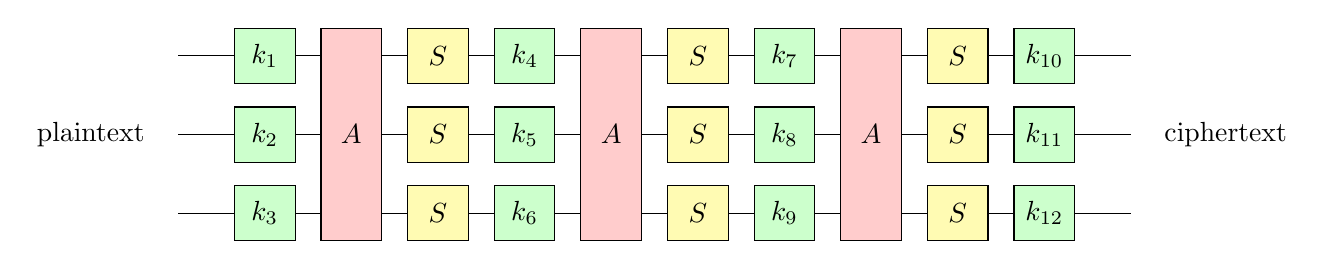
\begin{tikzpicture}[xscale=1.1,
      a/.style={fill=red!20},
      s/.style={fill=yellow!30},
      k/.style={fill=green!20}]
      \draw (0,2) -- (11,2);
      \draw (0,1) node[left=2ex]{plaintext} -- (11,1) node[right=2ex]{ciphertext};
      \draw (0,0) -- (11,0);
      \draw[k] (1,2) +(-0.35,-0.35) rectangle node{$k_1$} +(0.35,0.35);
      \draw[k] (1,1) +(-0.35,-0.35) rectangle node{$k_2$} +(0.35,0.35);
      \draw[k] (1,0) +(-0.35,-0.35) rectangle node{$k_3$} +(0.35,0.35);
      \draw[a] (2,0) +(-0.35,-0.35) rectangle node{$A$} +(0.35,2.35);
      \draw[s] (3,2) +(-0.35,-0.35) rectangle node{$S$} +(0.35,0.35);
      \draw[s] (3,1) +(-0.35,-0.35) rectangle node{$S$} +(0.35,0.35);
      \draw[s] (3,0) +(-0.35,-0.35) rectangle node{$S$} +(0.35,0.35);
      \draw[k] (4,2) +(-0.35,-0.35) rectangle node{$k_4$} +(0.35,0.35);
      \draw[k] (4,1) +(-0.35,-0.35) rectangle node{$k_5$} +(0.35,0.35);
      \draw[k] (4,0) +(-0.35,-0.35) rectangle node{$k_6$} +(0.35,0.35);
      \draw[a] (5,0) +(-0.35,-0.35) rectangle node{$A$} +(0.35,2.35);
      \draw[s] (6,2) +(-0.35,-0.35) rectangle node{$S$} +(0.35,0.35);
      \draw[s] (6,1) +(-0.35,-0.35) rectangle node{$S$} +(0.35,0.35);
      \draw[s] (6,0) +(-0.35,-0.35) rectangle node{$S$} +(0.35,0.35);
      \draw[k] (7,2) +(-0.35,-0.35) rectangle node{$k_7$} +(0.35,0.35);
      \draw[k] (7,1) +(-0.35,-0.35) rectangle node{$k_8$} +(0.35,0.35);
      \draw[k] (7,0) +(-0.35,-0.35) rectangle node{$k_9$} +(0.35,0.35);
      \draw[a] (8,0) +(-0.35,-0.35) rectangle node{$A$} +(0.35,2.35);
      \draw[s] (9,2) +(-0.35,-0.35) rectangle node{$S$} +(0.35,0.35);
      \draw[s] (9,1) +(-0.35,-0.35) rectangle node{$S$} +(0.35,0.35);
      \draw[s] (9,0) +(-0.35,-0.35) rectangle node{$S$} +(0.35,0.35);
      \draw[k] (10,2) +(-0.35,-0.35) rectangle node{$k_{10}$} +(0.35,0.35);
      \draw[k] (10,1) +(-0.35,-0.35) rectangle node{$k_{11}$} +(0.35,0.35);
      \draw[k] (10,0) +(-0.35,-0.35) rectangle node{$k_{12}$} +(0.35,0.35);
  \end{tikzpicture}
\end{center}
\end{definition}

Note that the three basic steps (key mixing, diffusion, and S-box
application) are repeated several times; each such repetition is
called a \textbf{round}%
\index{cipher!round}%
\index{rounds of a cipher} of the block cipher.  The more rounds a
block cipher has, the better its diffusion and non-linearity
properties. The final round is short: it only consists of a key
mixing step, with no final diffusion or S-box application. The reason
is that performing a final diffusion and S-box application would not
add anything to the security of the cipher. An attacker could simply
undo these last two steps, since they do not depend on the key.

The matrix $A$ is called the \textbf{diffusion matrix}%
\index{diffusion matrix}%
\index{matrix!diffusion}%
\index{cipher!diffusion matrix} of the cipher. Note that, unlike for
the Hill cipher, the matrix $A$ is fixed once and for all and is not
part of the key. Instead, the key consists of scalars that are added
to the current block at the beginning of each round.

\begin{example}{Toy block cipher: encryption}{toy-block-cipher-encryption}
  Encrypt the message ``I like math'' using the block cipher of
  Definition~\ref{def:toy-block-cipher} and the key
  $1,1,3,3,5,5,7,7,9,9,11,11$.
\end{example}

\begin{solution}
  We first represent the plaintext as a sequence of blocks, padding
  the final block with zeros:
  \begin{equation*}
    \mbox{Plaintext blocks:}\quad
    (9,0,12),\
    (9,11,5),\
    (0,13,1),\
    (20,8,0).
  \end{equation*}
  To encrypt the first block, we start with the vector
  $\startmat{c}9,0,12\stopmat^T$ and apply the following steps:

  \noindent{\bf Round 1:}
  \begin{itemize}
  \item Key mixing: the first three components of the key are
    $1,1,3$. We add them to the plaintext.
    \begin{equation*}
      \startmat{c} 9 \\ 0 \\ 12 \stopmat
      +
      \startmat{c} 1 \\ 1 \\ 3 \stopmat
      ~=~
      \startmat{c} 10 \\ 1 \\ 15 \stopmat.
    \end{equation*}
  \item Diffusion: multiply by the matrix $A$.
    \begin{equation*}
      \startmat{ccc}
        1 & 2 & 3 \\
        3 & 1 & 2 \\
        2 & 3 & 1 \\
      \stopmat
      \startmat{c} 10 \\ 1 \\ 15 \stopmat
      ~=~
      \startmat{c} 28 \\ 3 \\ 9 \stopmat.
    \end{equation*}
  \item S-box application: apply the S-box to each component of the
    vector.
    \begin{equation*}
      \startmat{c} S(28) \\ S(3) \\ S(9) \stopmat
      ~=~
      \startmat{c} 8 \\ 2 \\ 18 \stopmat.
    \end{equation*}
  \end{itemize}

  \noindent{\bf Round 2:}
  \begin{itemize}
  \item Key mixing: the next three components of the key are
    $3,5,5$.
    \begin{equation*}
      \startmat{c} 8 \\ 2 \\ 18 \stopmat
      +
      \startmat{c} 3 \\ 5 \\ 5 \stopmat
      ~=~
      \startmat{c} 11 \\ 7 \\ 23 \stopmat.
    \end{equation*}
  \item Diffusion:
    \begin{equation*}
      \startmat{ccc}
        1 & 2 & 3 \\
        3 & 1 & 2 \\
        2 & 3 & 1 \\
      \stopmat
      \startmat{c} 11 \\ 7 \\ 23 \stopmat
      ~=~
      \startmat{c} 7 \\ 28 \\ 8 \stopmat.
    \end{equation*}
  \item S-box application:
    \begin{equation*}
      \startmat{c} S(7) \\ S(28) \\ S(8) \stopmat
      ~=~
      \startmat{c} 26 \\ 8 \\ 16 \stopmat.
    \end{equation*}
  \end{itemize}

  \noindent{\bf Round 3:}
  \begin{itemize}
  \item Key mixing: the next three components of the key are
    $7,7,9$.
    \begin{equation*}
      \startmat{c} 26 \\ 8 \\ 16 \stopmat
      +
      \startmat{c} 7 \\ 7 \\ 9 \stopmat
      ~=~
      \startmat{c} 4 \\ 15 \\ 25 \stopmat.
    \end{equation*}
  \item Diffusion:
    \begin{equation*}
      \startmat{ccc}
        1 & 2 & 3 \\
        3 & 1 & 2 \\
        2 & 3 & 1 \\
      \stopmat
      \startmat{c} 4 \\ 15 \\ 25 \stopmat
      ~=~
      \startmat{c} 22 \\ 19 \\ 20 \stopmat.
    \end{equation*}
  \item S-box application:
    \begin{equation*}
      \startmat{c} S(22) \\ S(19) \\ S(20) \stopmat
      ~=~
      \startmat{c} 6 \\ 15 \\ 10 \stopmat.
    \end{equation*}
  \end{itemize}

  \noindent{\bf Round 4 (the final round is abbreviated):}
  \begin{itemize}
  \item Key mixing: the next three components of the key are
    $9,11,11$.
    \begin{equation*}
      \startmat{c} 6 \\ 15 \\ 10 \stopmat
      +
      \startmat{c} 9 \\ 11 \\ 11 \stopmat
      ~=~
      \startmat{c} 15 \\ 26 \\ 21 \stopmat.
    \end{equation*}
  \end{itemize}
  Therefore, the first ciphertext block is $(15,26,21)$. We repeat the
  same procedure with the remaining plaintext blocks, and obtain the
  following ciphertext blocks:
  \begin{equation*}
    \mbox{Ciphertext blocks:}\quad
    (15,26,21),\
    (7,24,1),\
    (2,16,23),\
    (7,20,22).
  \end{equation*}
  The corresponding ciphertext is $\q{OZUGXABPWGTV}$.
\end{solution}

Are ciphers like this actually used in the real world? The answer
is yes. While the cipher of Definition~\ref{def:toy-block-cipher} is
greatly simplified, it has the same basic structure as modern
real-world block ciphers (such as AES, the Advanced Encryption
Standard). Naturally, these real-world ciphers differ in some details,
such as the alphabet size, the block size, the number of rounds, the
design of the S-boxes, the way the key is computed, and the precise
order in which the operations are applied. However, their basic
structure is very similar to our toy cipher, and indeed, all such
ciphers rely on key mixing, diffusion, and non-linear S-boxes as
their key components.

For example, AES uses an alphabet size of $256$ instead of $29$ (i.e.,
it operates on bytes%
\index{byte}, rather than elements of $\Z_{29}$). Although $\Z_{256}$
is not a field (because $256$ is not prime), it nevertheless turns out
that there exists a field with $256$ elements, and AES uses it for its
algebraic operations. Our toy cipher's block size of $3$ is much too
small to achieve effective diffusion; modern real-world ciphers use
block sizes between $16$ and $32$ bytes ($128$ to $256$ bits). The
design of the S-boxes is a bit of a black art; at minimum, they must
be designed to withstand two common types of cryptanalysis known as
\textbf{linear cryptanalysis}%
\index{cryptanalysis!linear}%
\index{linear cryptanalysis} and \textbf{differential cryptanalysis}%
\index{cryptanalysis!differential}%
\index{differential cryptanalysis}.  Among other things, this means
that the S-box should be ``as far from linear'' as possible.

A detailed discussion of the design and cryptanalysis of modern block
ciphers is far beyond the scope of this book, but we hope that you
have gotten a taste of this fascinating subject, and the role that
linear algebra over finite fields plays in it.


\end{document}